\documentclass{article}
\usepackage[T2A]{fontenc} 
\usepackage[utf8]{inputenc} 
\usepackage[english,russian]{babel}
\usepackage{graphicx} 
\usepackage{amsmath}
\usepackage{amsfonts} 
\usepackage{titlesec}
\usepackage{listings}

\usepackage{titling} 
\usepackage{geometry} 
\usepackage{pgfplots}
\pgfplotsset{compat=1.9}
\usepackage{xcolor}
\definecolor{darkgreen}{RGB}{0,100,0}

\lstset{
  language=Python,
  basicstyle=\ttfamily,
  keywordstyle=\color{darkgreen},
  stringstyle=\color{purple},
  commentstyle=\color{green},
  morecomment=[l][\color{magenta}]{\#},
  frame=single, 
  showspaces=false, 
  showstringspaces=false, 
  numbers=left, 
  numberstyle=\tiny,
}

\titleformat{\section}
  {\normalfont\Large\bfseries}{\thesection}{1em}{}
\titleformat{\subsection}
  {\normalfont\large\bfseries}{\thesubsection}{1em}{}

\setlength{\droptitle}{-6em} 
\title{Отчет по лабораторной работе № 1 \\ Вариант № 3}
\author{Винницкая Дина Сергеевна}
\date{Группа: Б9122-02-03-01сцт}

\geometry{a4paper, margin=2cm}

\begin{document}

\maketitle
\section*{Цель работы}
\begin{enumerate}
    \item Построить интерполяционный многочлен Лагранжа для заданной функции.
    \item Построить таблицу абсолютной и относительной погрешностей остаточного члена для каждой $n$.
    \item Построить график зависимостей $\Delta f_n(n)$, $r_n(n)$.
    \item Сделать вывод.
\end{enumerate}

\section*{Входные данные:}
\begin{enumerate}

    \item \textbf{Функция:} $y=x^2 + \ln(x) - 4$
    \item \textbf{[a;b]:} $[1.5,2.0]$
    \item $n \in {3, 5, 10, 20, 30, 40, 50, 60, 70, 80, 90, 100} $
    
\end{enumerate}

\section*{Ход работы:}

\section{Используемые библиотеки}
Для реализации необходимой программы используются следующие библиотеки языка Python:

\begin{itemize}
    \item \textbf{numpy} - библиотека для работы с массивами, векторами и матрицами, включающая функции для линейной алгебры, преобразования Фурье и генерации псевдослучайных чисел.
    
    \item \textbf{math} - модуль для выполнения математических операций, таких как вычисление факториала и другие математические функции.
    
    \item \textbf{pandas} - библиотека для обработки и анализа данных, предоставляющая удобные структуры данных и операции для их анализа.
    
    \item \textbf{matplotlib} - библиотека для визуализации данных, позволяющая создавать различные виды графиков, диаграмм и других визуальных элементов.
\end{itemize}

\begin{lstlisting}
from numpy import linspace
from math import factorial
import pandas as pd
import numpy as np
\end{lstlisting}

\section{Определение функции и нахожение производной}
\begin{lstlisting}[language=Python]
def function(x: float):
    return x ** 2 + np.log(x) - 4
    
def derivative_function(x: float, n: int = 2) -> float:
    return 2 - 1 / (x ** 2)

value_range = [3, 5, 10, 20, 30, 40, 50, 60, 70, 80, 90, 100]

graph_range = (1.5, 2.0)
\end{lstlisting}

В коде представлено определение двух функций, одна из которых - исходная функция, вторая же, представляет собой ее производную, списка точек и кортежа значений заданного промежутка.

\section{Графическое отображение функции}

\begin{figure}[h]
    \centering
    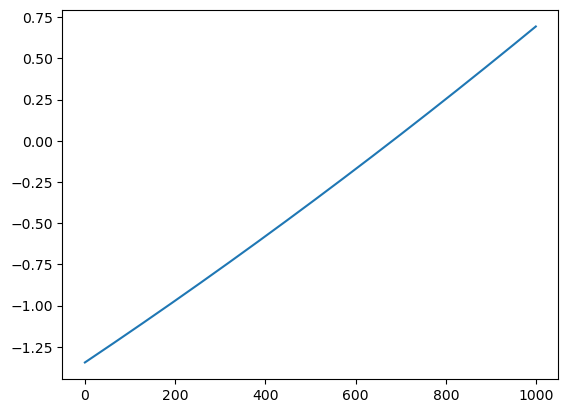
\includegraphics[width=0.5\textwidth]{output.png}
    \caption{Отображение функции}
    \label{fig:my_label}
\end{figure}

\begin{lstlisting}[language=Python]
import matplotlib.pyplot as plt

plt.plot(function(linspace(*graph_range, num=10 ** 3)))
\end{lstlisting}


\section{Реализация полинома Лагранжа}

\begin{lstlisting}[language=Python]
def generate_points(rng: tuple[float, float], count_points: int, function)
-> list[tuple[float, float]]:
    
    result = []
    for current_position in linspace(*rng, count_points):
        result.append((current_position, function(current_position)))
    return result

def lagrange_interpolation(bp: float, points: list[tuple[float, float]]) 
-> float:
    
    count_points = len(points)
    result = 0
    for k, point in enumerate(points):
        multiply = point[1]
        for j in range(0, k - 1 + 1):
            x = points[j][0]
            multiply *= ((bp - x) / (point[0] - x))
        for i in range(k + 1, count_points):
            x = points[i][0]
            multiply *= ((bp - x) / (point[0] - x))
        result += multiply
    return result


    
\end{lstlisting}

\begin{itemize}
\item Функция \texttt{lagrange\_interpolation} принимает базовую точку \texttt{bp} и список кортежей значений \texttt{points}, и возвращает значение интерполяции методом Лагранжа. Внутри функции выполняется итерация по всем точкам из списка \texttt{points}. Для каждой точки выполняются вычисления, используя формулу интерполяции Лагранжа, и результаты суммируются для получения окончательного значения интерполяции. 
\end{itemize}

\section{Вычисление ошибок}
\textbf{\large{Норма}}

\begin{lstlisting}[language=Python]
def calculate_max_absolute_value(function, rng: tuple[float, float],
*args) -> float:

    return max(abs(function(linspace(*rng, num=10 ** 3), *args)))
    
\end{lstlisting}

\begin{itemize}
\item Функция \texttt{calculate\_max\_absolute\_value} принимает функцию \texttt{function}, диапазон \texttt{rng} и дополнительные аргументы \texttt{*args}, и возвращает максимальное абсолютное значение функции в указанном диапазоне. В этой функции используется функция \texttt{linspace} для генерации значений в указанном диапазоне, после чего вычисляется максимальное абсолютное значение функции с помощью функции \texttt{max}.
\end{itemize}

\textbf{\large{Относительная ошибка}}

\begin{lstlisting}[language=Python]
def relative_error(abs_error: float, func_norm: float) -> float:

    return (abs_error / func_norm) * 100
    
\end{lstlisting}

\begin{itemize}
\item Функция \texttt{relative\_error} принимает абсолютную ошибку \texttt{abs\_error} и норму функции \texttt{func\_norm} в качестве входных данных. Она возвращает относительную ошибку, которая вычисляется как отношение абсолютной ошибки к норме функции, умноженное на 100.
\end{itemize}

\textbf{Графическое представление}

\begin{lstlisting}[language=Python]
rel_df.plot(xticks=value_range, yticks=range(0, 100 + 1, 10),
xlabel="n",ylabel="%")
    
\end{lstlisting}

\begin{figure}[h]
    \centering
    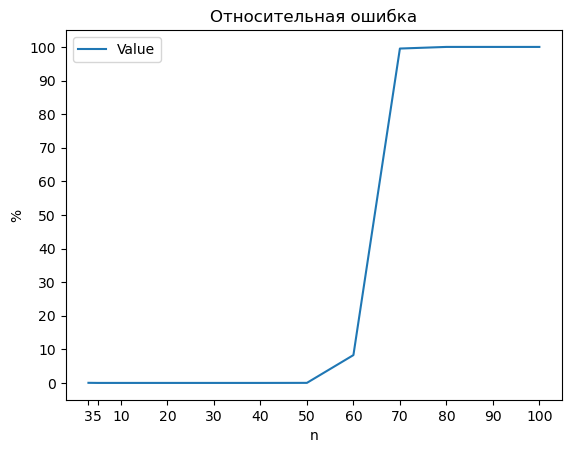
\includegraphics[width=0.5\textwidth]{output2.png}
    \label{fig:my_label}
\end{figure}


\textbf{\large{Теоретическая ошибка}}

\begin{lstlisting}[language=Python]
def theoretical_error(count_points: int, range_tuple: tuple[float, float])
-> float:
    
    return (calculate_max_absolute_value(derivative_function, range_tuple,
    count_points + 1) / factorial(count_points + 1)) * (
            (range_tuple[1] - range_tuple[0]) ** (count_points + 1))
    
\end{lstlisting}

\begin{itemize}
\item Функция \texttt{theoretical\_error} принимает количество точек
\texttt{count\_points} и диапазон значений 
\texttt{range\_tuple} в виде кортежа. Она возвращает теоретическую ошибку для указанного количества точек. Внутри функции используется функция \texttt{calculate\_max\_absolute\_value} для вычисления максимального абсолютного значения производной функции \texttt{derivative\_function} и факториал для указанного количества точек, чтобы получить теоретическую ошибку.
\end{itemize}

\textbf{Графическое представление}

\begin{lstlisting}[language=Python]
abs_df.plot(xticks=value_range, xlabel="n")
    
\end{lstlisting}

\begin{figure}[h]
    \centering
    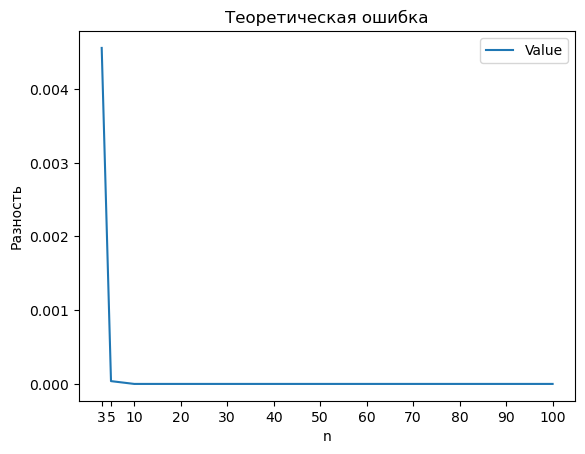
\includegraphics[width=0.5\textwidth]{output3.png}
    \label{fig:my_label}
\end{figure}


\section{Основной цикл}
\begin{lstlisting}[language=Python]
absolute_error_arr = []
relative_error_arr = []
theoretical_error_arr = []

for num_points in value_range:

    current_points = generate_points(graph_range, num_points, function)
    norm = calculate_max_absolute_value(function, graph_range)
    
    lagrange_norm = calculate_max_absolute_value(lagrange_interpolation,
    graph_range, current_points)
    
    absolute_error = max(abs(lagrange_interpolation(linspace(*graph_range,
    num=10 ** 3), current_points) - function(
        linspace(*graph_range, num=10 ** 3))))
        
    der_e = calculate_max_absolute_value(derivative_function, graph_range)
    rel_e = relative_error(absolute_error, lagrange_norm)
    ter_e = theoretical_error(num_points, graph_range)

    absolute_error_arr.append(absolute_error)
    relative_error_arr.append(rel_e)
    theoretical_error_arr.append(ter_e)

abs_df = pd.DataFrame(absolute_error_arr, value_range, columns=["Value"])

rel_df = pd.DataFrame(relative_error_arr, value_range, columns=["Value"])

ter_df = pd.DataFrame(theoretical_error_arr, value_range, columns=["Value"])

total_df = pd.DataFrame({"Absolute error": absolute_error_arr,
                         "Relative error": relative_error_arr,
                         "Theoretical error": theoretical_error_arr},
                        index=value_range)
total_df.to_csv("ansv.csv")


    
\end{lstlisting}

\begin{itemize}
\item Для каждого значения \texttt{num\_points} из набора значений \texttt{value\_range}:
\begin{itemize}
    \item Генерация точек \texttt{current\_points} с помощью функции \texttt{generate\_points} для указанного диапазона \texttt{graph\_range} и количества точек \texttt{num\_points} с использованием функции \texttt{function}.
    
    \item Вычисление нормы \texttt{norm} с помощью функции \texttt{calculate\_max\_absolute\_value} для функции \texttt{function} и заданного диапазона \texttt{graph\_range}.
    
    \item Вычисление нормы лагранжевой интерполяции \texttt{lagrange\_norm} с помощью функции \\ \texttt{calculate\_max\_absolute\_value} для лагранжевой интерполяции \texttt{lagrange\_interpolation}, указанного диапазона \texttt{graph\_range} и точек \texttt{current\_points}.
    
    \item Вычисление абсолютной ошибки \texttt{absolute\_error} как максимального значения модуля разницы между значением лагранжевой интерполяции и значением функции на тысяче равномерно распределенных точках в заданном диапазоне \texttt{graph\_range}.
    
    \item Вычисление нормы производной \texttt{der\_e} с использованием функции \texttt{calculate\_max\_absolute\_value} для производной функции \texttt{derivative\_function} в указанном диапазоне \texttt{graph\_range}.
    
    \item Вычисление относительной ошибки \texttt{rel\_e} с использованием функции \texttt{relative\_error} на основе абсолютной ошибки и нормы лагранжевой интерполяции.
    
    \item Вычисление теоретической ошибки \texttt{ter\_e} с использованием функции \texttt{theoretical\_error} для указанного количества точек \texttt{num\_points} и диапазона \texttt{graph\_range}.
    
    \item Добавление вычисленных значений абсолютной ошибки, относительной
    ошибки и теоретической ошибки в соответствующие списки \texttt{absolute\_error\_arr}, \\ \texttt{relative\_error\_arr} и \texttt{theoretical\_error\_arr} соответственно.
\end{itemize}

\item Создание трех \texttt{DataFrame} с использованием библиотеки \texttt{pandas} для абсолютной ошибки, относительной ошибки и теоретической ошибки под названиями \texttt{abs\_df}, \texttt{rel\_df} и \texttt{ter\_df}, соответственно. Эти \texttt{DataFrame} содержат вычисленные значения, а индексы установлены равными значениям из \texttt{value\_range}.

\item Построение графиков для каждой ошибки с использованием функции \texttt{plot} из библиотеки \texttt{pandas}, где каждый график имеет заголовок, оси и отметки на осях, основанные на соответствующих значениях из \texttt{value\_range}.

\end{itemize}

\textbf{\large{Абсолютная ошибка}}
\begin{lstlisting}[language=Python]
ter_df.plot(xticks=value_range, xlabel="n")
\end{lstlisting}
\textbf{Графическое представление}
    

\begin{figure}[h]
    \centering
    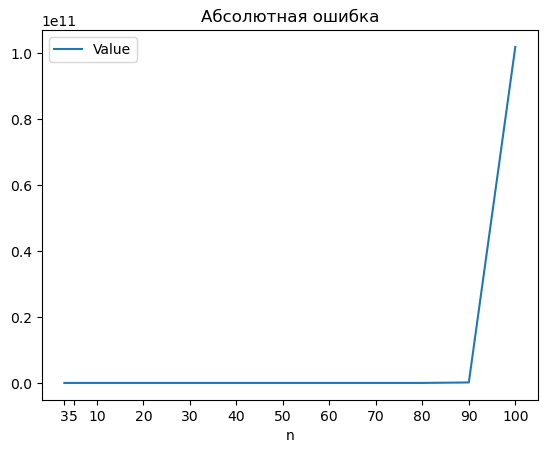
\includegraphics[width=0.5\textwidth]{output1.png}
    \label{fig:my_label}
\end{figure}

\section{Таблица}

\begin{itemize}
\item В результате работы цикла создается \texttt{csv} файл, содержащий в каждой
строке количество точек, а также значения ошибок при этом количестве точек. 
\end{itemize}

\begin{array}{|c|c|c|c|}
\hline
\text{ n } & \text{  Абсолютная ошибка  } & \text{  Относительная ошибка  } & \text{  Теоретическая ошибка  } \\
\hline
3 & 0.0004041198030879656 & 0.030056475702117818 & 0.004557291666666667 \\
5 & 1.5256277570152577 \times 10^{-6} & 0.00011346881112684361 & 3.7977430555555556 \times 10^{-5} \\
10 & 5.257128066205041 \times 10^{-12} & 3.9099975001823635 \times 10^{-10} & 2.1406830895763187 \times 10^{-11} \\
20 & 6.290523657526137 \times 10^{-13} & 4.678587142260786 \times 10^{-11} & 1.6332934790103295 \times 10^{-26} \\
30 & 3.5273739484864564 \times 10^{-10} & 2.6234900780620463 \times 10^{-8} & 9.91029116659731 \times 10^{-44} \\
40 & 4.1140015138996233 \times 10^{-7} & 3.0597952784334175 \times 10^{-5} & 2.3789170643336584 \times 10^{-62} \\
50 & 0.00022682959886166643 & 0.016870488094400032 & 5.010294122165272 \times 10^{-82} \\
60 & 0.11674814466636829 & 8.28336936102891 & 1.4952149433536201 \times 10^{-102} \\
70 & 140.79557454487764 & 99.51802119595312 & 8.71455012283797 \times 10^{-124} \\
80 & 77993.4186208717 & 100.00088295864624 & 1.248520445119785 \times 10^{-145} \\
90 & 139505887.07198614 & 99.99999950636955 & 5.227948020826171 \times 10^{-168} \\
100 & 101879015502.40543 & 99.99999999932184 & 7.322905978848986 \times 10^{-191} \\
\hline
\end{array}

\section{Вывод}

\begin{itemize}
\item В результате проделанной работы был реализована функция полинома Лагранжа, а заключении необходимо проанализировать поведение графиков ошибок: 
\begin{itemize}
    \item Можно сделать вывод о том, что до $11$ точек абсолютная ошибка стремилась к 0, но после она начала стремится к $+\infty$.
    \item Так же исходя из представленного ранее графика можно понять, что теоретическая ошибка стремится к 0.
    \item Обратя внимание на график относительной ошибки, можно прийти к выводу о том, что она стремится к $100\%$.

\end{itemize}


\thispagestyle{empty} 
\newpage
\mbox{}
\thispagestyle{empty} 
\newpage
 
\end{document}
